\documentclass{beamer}
\usetheme{ConnectivityLab}
\usepackage{times}
\usepackage{graphicx}
\usepackage{verbatim}
\usepackage{outlines}
\usepackage{fancyhdr}
\usepackage{subfigure}
\usepackage{cancel}
\usepackage{bibentry}
\usepackage{varwidth}
\usepackage{etoolbox}
\usepackage{epstopdf}

%%%%%%%%%%%%%%%%%%%%%%%%%%%%%%%%%%%%%%%%%%%%%%%%%%%%%%
%%%%%%%%%%%%%%%%%%%%%%%%%%%%%%%%%%%%%%%%%%%%%%%%%%%%%%

\title {
    Priority-Based Random Access Control Mechanism for M2M Communications \cite{Guan16}
}
\author {
    Yin-Hong Hsu
}
\date {
    09/01, 2017 %\today
}

%%%%%%%%%%%%%%%%%%%%%%%%%%%%%%%%%%%%%%%%%%%%%%%%%%%%%%
%%%%%%%%%%%%%%%%%%%%%%%%%%%%%%%%%%%%%%%%%%%%%%%%%%%%%%

\begin{document}
\begin{frame}
    \titlepage
\end{frame}

\begin{frame}{Outline}
    \tableofcontentsgather
    \tableofcontents
\end{frame}

\section{Introduction}
\begin{frame}{Introduction}
\begin{itemize}
    \item {{PBRA} mechanism}
    \item {dynamically control the UEs' access}
    \item {according to the number of access attempts and their priority}
\end{itemize}
\end{frame}
\begin{frame}{Random Access Procedure}
\begin{figure}[t]
    \centering
    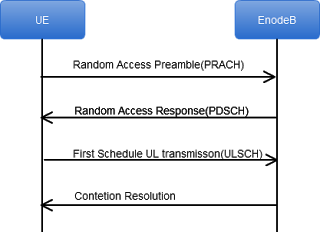
\includegraphics[width=0.9\textwidth]{figures/rap.png}
    \setbeamerfont{caption}{size=\tiny}
\end{figure}
\end{frame}
\begin{frame}{Access Class Barring}
\begin{figure}[t]
    \centering
    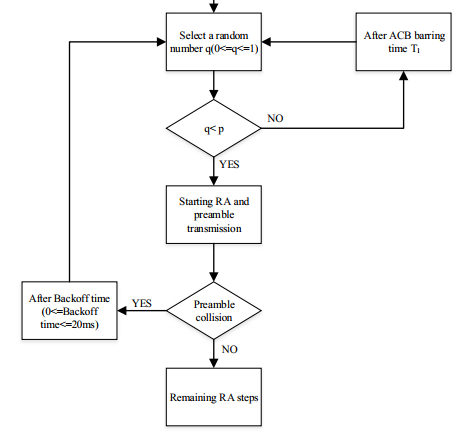
\includegraphics[width=0.7\textwidth]{figures/acb.png}
    \setbeamerfont{caption}{size=\tiny}
\end{figure}
\end{frame}
\begin{frame}{Priority Classification}
    \begin{itemize}
        \item {Classify according to their delay sensibility}
        \item {high priority}
        \item {medium priority}
        \item {low priority}
    \end{itemize}
\end{frame}

\section{Mechanism}

\begin{frame} {Preamble split}
    \begin{itemize}
        \item \textbf{Seperate 54 preambles into 2 groups}
        \item \textbf{Group 1: 1 to S}
        \item \textbf{Group 2: S+1 to 54}
        \item \textbf{S will rise while the congestion in Group 1 increase} 
    \end{itemize}
\end{frame}
\begin{frame} {Preamble split}
    \begin{figure}[t]
    \centering
    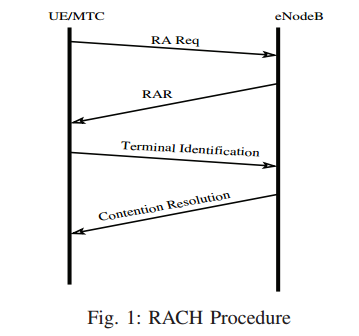
\includegraphics[width=0.9\textwidth]{figures/p1.png}
    \setbeamerfont{caption}{size=\tiny}
\end{figure}
\end{frame}
\begin{frame} {Estimation and Strategy }
    \begin{itemize}
        \item \textbf{Three steps}
        \begin{itemize}
            \item[-] Initialization
            \begin{itemize}
                \item[+] set all variable to 0
            \end{itemize}
            \item[-] Detection
            \begin{itemize}
                \item[+] calculate the total number of conflicted preambles
            \end{itemize}
            \item[-] Implementation
            \begin{itemize}
                \item[+] calculate the average preamble collision ratio of each group
                \item[+] Ci: collision ratio of group i
                \item[+] $S_{i} = S_{i-1} \cdot  \left \lfloor \left ( C1_{i-1}-0.05 \right )\cdot b \right \rfloor$
                \item[+] $a_{i} = 1 - C2 \cdot g$
            \end{itemize}
        \end{itemize}
         
    \end{itemize}
\end{frame}
\begin{frame} {Estimation and Strategy }
    \begin{figure}[t]
    \centering
    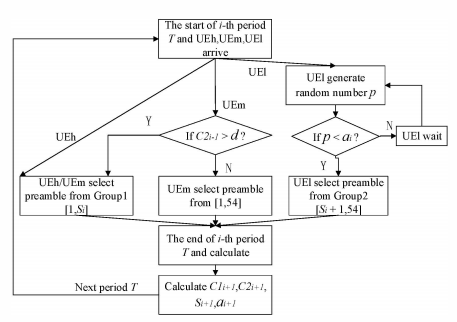
\includegraphics[width=0.9\textwidth]{figures/p2.png}
    \setbeamerfont{caption}{size=\tiny}
\end{figure}
\end{frame}
%%%%%%%%%%%%%%%%%%%%%%%%%%%%%%%%%%%%%%%%%%%%%%%%%%%%%%
%%%%%%%%%%%%%%%%%%%%%%%%%%%%%%%%%%%%%%%%%%%%%%%%%%%%%%

%%%%%%%%%%%%%%%%%%%%%%%%%%%%%%%%%%%%%%%%%%%%%%%%%%%%%%
%%%%%%%%%%%%%%%%%%%%%%%%%%%%%%%%%%%%%%%%%%%%%%%%%%%%%%
\section{Evaluation}

\begin{frame} {Success Probability\cite{Zangar16}}
    \begin{figure}[t]
    \centering
    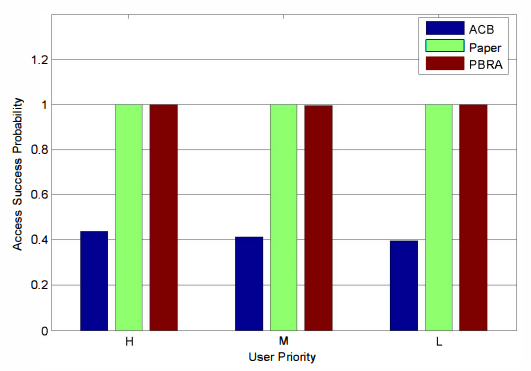
\includegraphics[width=0.9\textwidth]{figures/p3.png}
    \setbeamerfont{caption}{size=\tiny}
\end{figure}
\end{frame}
\begin{frame} {Access Delay\cite{Zangar16}}
    \begin{figure}[t]
    \centering
    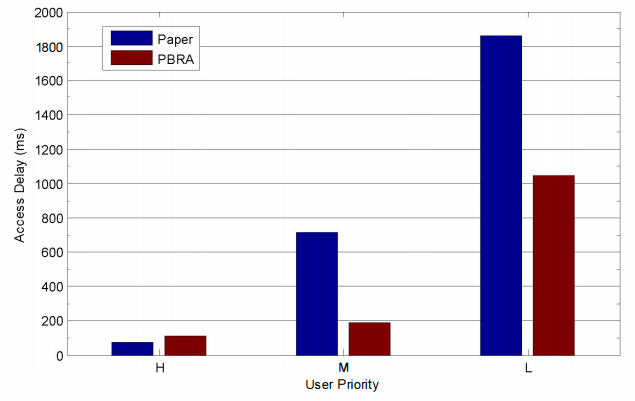
\includegraphics[width=0.9\textwidth]{figures/p4.png}
    \setbeamerfont{caption}{size=\tiny}
\end{figure}
\end{frame}
\begin{frame} {Number of Access Slot\cite{Zangar16}}
    \begin{figure}[t]
    \centering
    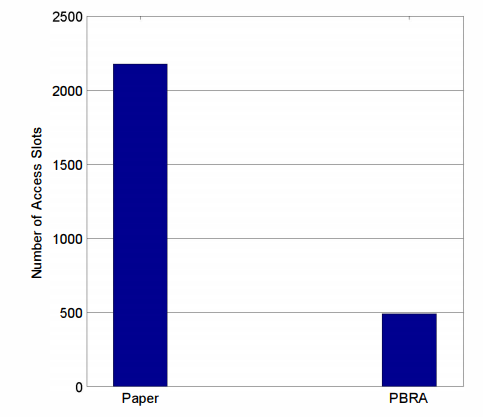
\includegraphics[width=0.7\textwidth]{figures/p5.png}
    \setbeamerfont{caption}{size=\tiny}
\end{figure}
\end{frame}


\section{References}
\calcreferencespagetotal % Calc your References Page total number
\begin{frame}[allowframebreaks]{References}
    \fontsize{9pt}{13}\selectfont
    \bibliographystyle{IEEEtran}
    \bibliography{IEEEabrv,Citation}
\end{frame}
\end{document}
